\input ../SlidePreamble
\input ../preamble


\begin{document}

{\Huge

  \centerline{\bf TTIC 31230, Fundamentals of Deep Learning}
  \bigskip
  \centerline{David McAllester, Winter 2019}
  \vfill
  \centerline{\bf Discrimination Loss}
  \vfill
  \centerline{\bf and Generative Adversarial Networks (GANs)}
\vfill
\vfill

\slide{Representing a Distribution with a Generator}
\centerline{$z\sim {\cal N}(0,I)$ \hspace{7em} $y\sim p_\Phi$}
\centerline{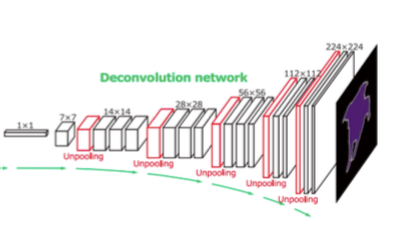
\includegraphics[width=6in]{../images/halfdeconv}}


\slidetwo{Generative Adversarial Nets}{Goodfellow et al., June 2014}

In a GAN the parameters $\Phi$ of a generator network are trained by the equation
{\color{red} $$\Phi^* = \argmin_\Phi {\cal L}_{\mathrm{Discr}}(\popd,p_\Phi).$$}

\vfill
Here ${\cal L}_{\mathrm{Discr}}(\popd,p_\Phi)$ is a ``discrimination loss'' --- the ability of a discriminator to distinguish the population distribution $\popd$ from
the generated model distribution $p_\Phi$.

\slide{Classification Discrimination}

\vfill
In the original GAN paper (Goodfellow et al.), and in current practice, the discriminator is a classifier that classifies samples as either being from the population or being from the model.

\vfill
Let ${\color{red} p \uplus q}$ be the distribution defined by flipping an unbiased coin and, if heads, returning {\color{red} $(1,y)$} with
{\color{red} $y \sim p$} and, if tails, returning {\color{red} $(-1,y)$} with {\color{red} $y \sim q$}.


{\color{red} $${\cal L}_{\mathrm{Discr}}(p,q) = \max_\Psi\;E_{(i,y) \sim p \uplus q}\;\ln P_\Psi(i|y)$$}

\slide{Assuming Universality of $\Psi$}

$$\Phi^* = \argmin_\Phi {\cal L}_{\mathrm{Discr}}(\popd,p_\Phi).$$

\begin{eqnarray*}
{\cal L}_{\mathrm{Discr}}(\popd,p_\Psi) & = & \max_\Psi\;E_{(i,y) \sim \popd \uplus p_\Phi}\;\ln P_\Psi(i|y)
\end{eqnarray*}

{\color{red} $$\Psi^* = \argmin_\Psi \;E_{(i,y) \sim \popd \uplus p_\Phi}\;- \ln P_\Psi(i|y)$$}

Assuming Universality for $\Psi$, {\color{red} $P_{\Psi^*}(i|y)$ equals the true probability $P_\Phi(i|y)$ defined by the distribution $\popd\uplus p_\Phi$}.


{\color{red} $$P_{\Psi^*}(i|y) = P_\Phi(i|y)$$}

\slide{Assuming Universality}

$$\Phi^* = \argmin_\Phi {\cal L}_{\mathrm{Discr}}(\popd,p_\Phi).$$

\begin{eqnarray*}
{\color{red} {\cal L}_{\mathrm{Discr}}(\popd,p_\Phi)} & = & E_{(i,y) \sim \popd \uplus p_\Phi}\;\ln P_{\Phi}(i|y) \\
\\
& = & {\color{red} -H(i|y)}
\end{eqnarray*}

The generator $\Phi$ is trying to maximize $H(i|y)$ which is achieved at $\ln 2$ (one bit) for $p_\Phi = \popd$.

\vfill
Assuming Universality of both $\Phi$ and $\Psi$ we have {\color{red} $p_{\Phi^*} = \popd$}.

\slide{Review of Binary Classification}

In the case of binary classification cross-entropy loss becomes the log loss of the margin

\begin{eqnarray*}
\Psi^* & = & \argmin_\Psi \;\expectsub{(i,y) \sim (\mathrm{Pop}\; \uplus \;P_\Phi)}{- \ln P_\Psi(i|y)} \\
\\
& = & \argmin_\Psi \expectsub{(i,y) \sim (\mathrm{Pop}\; \uplus \;P_\Phi)}{\;\;\;\ln(1 + e^{-m}}) \\
\\
m & = & i\;s_\Psi(y)
\end{eqnarray*}


\centerline{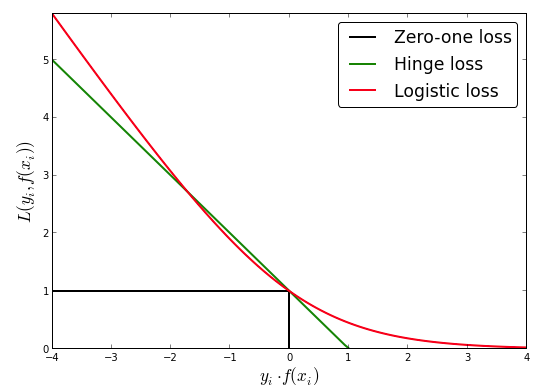
\includegraphics[height= 1.5in]{../images/logloss}}

\slide{Vanishing Gradients}

For $i = 1$ and $y \sim \popd$:
$$\Psi \;\pluseq \; \eta\;\frac{e^{-m}}{1 + e^{-m}}\;\nabla_\Psi \; s_\Psi(y) \;\;\approx 0 \;\mbox{for}\;m >> 1$$

\vfill
For $i = -1$ and $y \sim P_\Phi$:

$$\Psi \;\minuseq \; \eta\;\frac{e^{-m}}{1 + e^{-m}}\;\nabla_\Psi\;s_\Psi(y_\Phi(z)) \;\;\approx 0 \;\mbox{for}\;m >> 1$$

\vfill
$$\Phi \;\pluseq \; \eta\;\frac{e^{-m}}{1 + e^{-m}}\;\nabla_\Phi\; s_\Psi(y_\Phi(z)) \;\;\approx 0 \;\mbox{for}\;m >> 1$$

\vfill
The gradients vanish when the discriminator achieves large margins.

\slide{A Heuristic Patch}

Replace

$$\Phi \;\pluseq \; \eta\;\frac{e^{-m}}{1 + e^{-m}}\;\nabla_\Phi\; s_\Psi(y_\Phi(z)) \;\;\approx 0 \;\mbox{for}\;m >> 1$$

\vfill
with

$$\Phi \;\pluseq \; \eta\;\nabla_\Phi \; s_\Psi(y_\Phi(z))$$

\vfill
This allows the generator to recover.

\slidetwo{Generative Adversarial Nets}{Goodfellow et al., June 2014}
\centerline{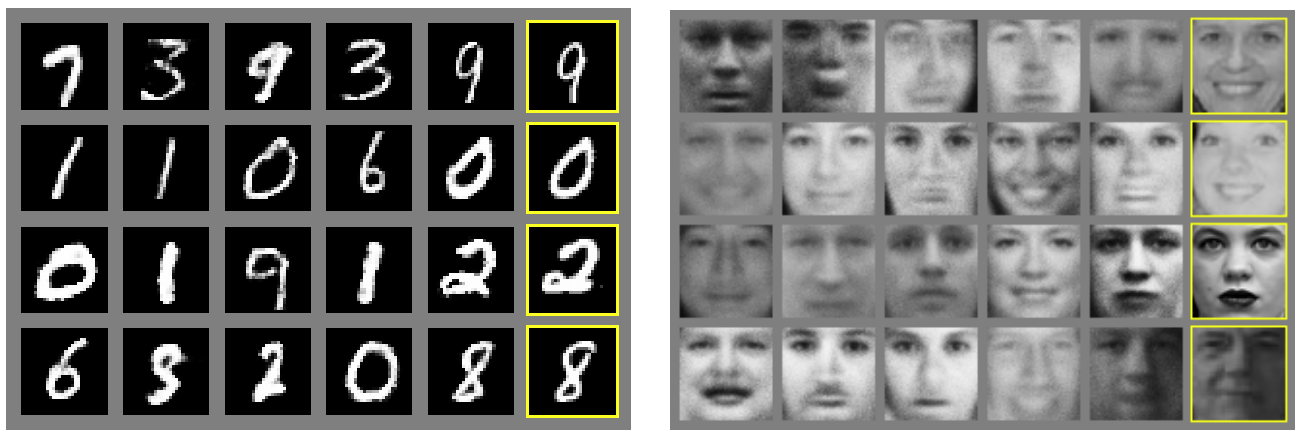
\includegraphics[width = 9in]{../images/GAN2014}}
The rightmost column (yellow boarders) gives the nearest neighbor in the training data to the adjacent column.

\slide{Assuming Universality of $\Psi$ Only}

\begin{eqnarray*}
{\color{red} - H(i|y)} & = & E_{(i,y) \sim (\popd\uplus p_\Phi)}\; \ln P(i|y) \\
\\
P(i|y) & = & \frac{p(i \wedge y)}{p(y)} \\
\\
\\
P(1|y) & = & \frac{\frac{1}{2}\popd(y)}{\frac{1}{2}\popd(y) + \frac{1}{2}p_\Phi(y)}
\end{eqnarray*}

\slide{Assuming Universality of $\Psi$ Only}

\begin{eqnarray*}
& & E_{(i,y) \sim (\popd\uplus p_\Phi)}\;\ln P(i|y) \\
\\
& = & \frac{1}{2} E_{y \sim \popd}\; \ln \frac{\frac{1}{2}\popd(y)}{\frac{1}{2}\popd(y) + \frac{1}{2} p_\Phi(y)} + \frac{1}{2} E_{y \sim p_\Phi}\;\ln \frac{\frac{1}{2}p_\Phi(y)}{\frac{1}{2}\popd(y) + \frac{1}{2}p_\Phi(y)} \\
\\
\\
& = & \frac{1}{2} \left(\;KL\left(\popd,\frac{\popd+p_\Phi}{2}\right),\;KL\left(p_\Phi,\frac{\popd+p_\Phi}{2}\right)\right) - \ln 2 \\
\\
& = & {\color{red} \mathrm{JSD}(\popd,p_\Phi) - \ln 2}
\end{eqnarray*}

\slide{Assuming Universality of $\Psi$ Only}

{\color{red} $$\Phi^* = \argmin_\Phi\;\mathrm{JSD}(\popd,p_\Phi)$$}

\slidetwo{Contrastive Discrimination}{Gutmann and Hyv\"{a}rinen, 2010}

Let {\color{red} $\popd\hookrightarrow p_\Phi^N$} be the distribution defined by drawing one ``positive'' from $\popd$ and $k$ IID negatives from $p_\Phi$;
then inserting the positive at a random position among the negatives; and returning $(i,y_1,\ldots,y_{N+1})$ where
$i$ is the index of the positive.

{\color{red} $${\cal L}_{\mathrm{Discr}}(\popd,p_\Phi)  = \max_\Psi\; E_{(i,y_1,\ldots,y_{N+1})\sim (\popd\hookrightarrow p_\Phi^N)} \; \ln P_\Psi(i|y_1,\ldots,y_{N+1})$$}

\slide{Contrastive Discrimination}

{\color{red} $$\Psi^* = \argmin_\Psi\; E_{(i,y_1,\ldots,y_{N+1})\sim (\popd\hookrightarrow p_\Phi^N)} \;- \ln P_\Psi(i|y_1,\ldots,y_{N+1})$$}

\vfill
Note that $\popd\hookrightarrow p_\Phi^1$ requires a choice between two $y$'s while $\popd\uplus p_\Phi$ classifies a single $y$ --- these are different.

\vfill
The contrastive task gets more difficult as $N$ gets larger.

\slide{Assuming Universality}

{\color{red} $$\Psi^* = \argmin_\Psi\; E_{(i,y_1,\ldots,y_{N+1})\sim (\popd\hookrightarrow p_\Phi^N)} \;- \ln P_\Psi(i|y_1,\ldots,y_{N+1})$$}

Assuming universality of $\Psi$ we get

{\color{red} $${\cal L}_{\mathrm{Discr}}(\Phi) = -H(i|y_1,\ldots y_{N+1})$$}

\vfill
The generator $\Phi$ is trying to maximize $H(i|y_1,\ldots,y_{N+1})$.

\vfill
The maximum is achieved at $\ln (N+1)$ for $p_\Phi = \popd$.

\slidetwo{Assuming Universality of a score function $s_\Psi$}{Gutmann and Hyv\"{a}rinen, 2010}


$$\Psi^* = \argmin_\Psi E_{(i,y_1,\ldots,y_{N+1}) \sim (\popd\hookrightarrow p_\Phi^N)} \;- \ln P_\Psi(i|y_1,\ldots,y_{N+1})$$
$$\mathrm{Assume:}\;\;\;\;{\color{red}P_\Psi(i|y_1,\ldots,y_{N+1}) \doteq \softmax_i s_\Psi(y_i)}$$

\vfill
{\color{red} Theorem}: Assuming universality:
\begin{eqnarray*}
P_{\Psi^*}(i|y_1,\ldots,y_{N+1}) & = & \softmax_i\;\; \ln \frac{\popd(y_i)}{p_\Phi(y_i)}
\end{eqnarray*}

And therefore:
\begin{eqnarray*}
{\color{red} \popd(y)} & {\color{red} =} & {\color{red} \softmax_y\;\;\; s_{\Psi^*}(y) - \ln p_\Phi(y)}\;\;\mbox{$Z$ must be estimated}
\end{eqnarray*}

\slide{Proof}
{\huge
\begin{eqnarray*}
{\color{red} P(i \;\mathrm{and}\;y_1,\ldots,y_{N+1})} & = & \frac{1}{N+1}\;\popd(y_i)\prod_{j \not = i}p_\Phi(y_j) \\
\\
& = & \alpha \frac{\popd(y_i)}{p_\Phi(y_i)},\;\;\;\alpha = \frac{1}{N+1} \prod_i p_\Phi(y_i) \\
\\
\\
{\color{red} P(i\;|\;y_1,\ldots y_{N+1})} & = & \frac{P(i\;\mbox{and} \; y_1,\ldots,y_{k+})}{\sum_i \;P(i \;\mbox{and}\; y_1,\ldots,y_{k+})} \\
\\
\\
& = & {\color{red} \softmax_i\; \left(\ln \frac{\popd(y_i)}{p_\Phi(y_i)}\right)}
\end{eqnarray*}
}


\slide{Assuming Universality of $s_\Psi$}


{\color{red} Theorem:}

\begin{eqnarray*}
P_{\Psi^*}(i|y_1,\ldots,y_{N+1}) & = & \softmax_i\;\; \ln \frac{\popd(y_i)}{p_\Phi(y_i)}
\end{eqnarray*}

\vfill
{\color{red} implies}
\begin{eqnarray*}
  && E_{(i,y_1,\dots,y_{N+1}) \sim \popd\hookrightarrow p_\Phi^N}\;\ln p_{\Psi^*}(i|y_1,\ldots,y_{N+1}) \\
  \\
  & \leq & \frac{N}{N+1}(KL(\popd,p_\Phi) + KL(p_\Phi,\popd)) + \ln \frac{1}{N+1}
\end{eqnarray*}

\vfill
Note that this upper bound holds with equality for $p_\Phi = \popd$.

\slide{Proof Part A.}

{\huge
 \begin{eqnarray*}
    & & E_{(i,y_1,\ldots,y_{N+1}) \sim \popd \hookrightarrow p_\Phi^N}\;\ln p_{\Psi^*}(i|y_1,\ldots,y_{N+1}) \\
    \\
    & = & E_{(i,y_1,\ldots,y_{N+1}) \sim \popd\hookrightarrow p_\Phi^N}\;\ln \left(\softmax_i \;\ln \frac{\popd(y_i)}{p_\Phi(y_i)}\right)[i] \\
    \\
    & = & E_{(i,y_1,\ldots,y_{N+1}) \sim \popd\hookrightarrow p_\Phi^N}\;\ln\frac{\popd(y_i)}{p_\Phi(y_i)} - \ln\left(\sum_i \frac{\popd(y_i)}{p_\Phi(y_i)} \right) \\
    \\
    & = & E_{(i,y_1,\ldots,y_{N+1}) \sim \popd\hookrightarrow p_\Phi^N}\;\ln\frac{\popd(y_i)}{p_\Phi(y_i)} - \ln\left(\frac{1}{N+1}\sum_i \frac{\popd(y_i)}{p_\Phi(y_i)} \right) - \ln\;(N+1)
  \end{eqnarray*}
}

\slide{Proof Part B.}
{\huge
 \begin{eqnarray*}
    & & E_{(i,y_1,\ldots,y_{N+1}) \sim \popd \hookrightarrow p_\Phi^N}\;\ln p_{\Psi^*}(i|y_1,\ldots,y_{N+1}) \\
    \\
    & = & E_{(i,y_1,\ldots,y_{N+1}) \sim \popd\hookrightarrow p_\Phi^N}\;\ln\frac{\popd(y_i)}{p_\Phi(y_i)} - \ln\left(\frac{1}{N+1}\sum_i \frac{\popd(y_i)}{p_\Phi(y_i)} \right) - \ln\;(N+1) \\
    \\
    & \leq & E_{(i,y_1,\ldots,y_{N+1}) \sim \popd\hookrightarrow p_\Phi^N}\;\ln\frac{\popd(y_i)}{p_\Phi(y_i)} - \frac{1}{N+1} \sum_i \ln\frac{\popd(y_i)}{p_\Phi(y_i)} - \ln\;(N+1) \\
    \\
    & = & \frac{N}{N+1} E_{y \sim \popd} \ln \frac{\popd(y)}{p_\Phi(y)} - \frac{N}{N+1} E_{y \sim p_\Phi} \ln \frac{\popd(y)}{p_\Phi(y)} - \ln\;(N+1) \\
    \\
    & = & \frac{N}{N+1}(KL(\popd,p_\Phi) + KL(p_\Phi,\popd)) - \ln\;(N+1) \\
  \end{eqnarray*}
}

\slidetwo{Unsupervised Representation Learning ... (DC GANS)}
{Radford et al., Nov. 2015}

\centerline{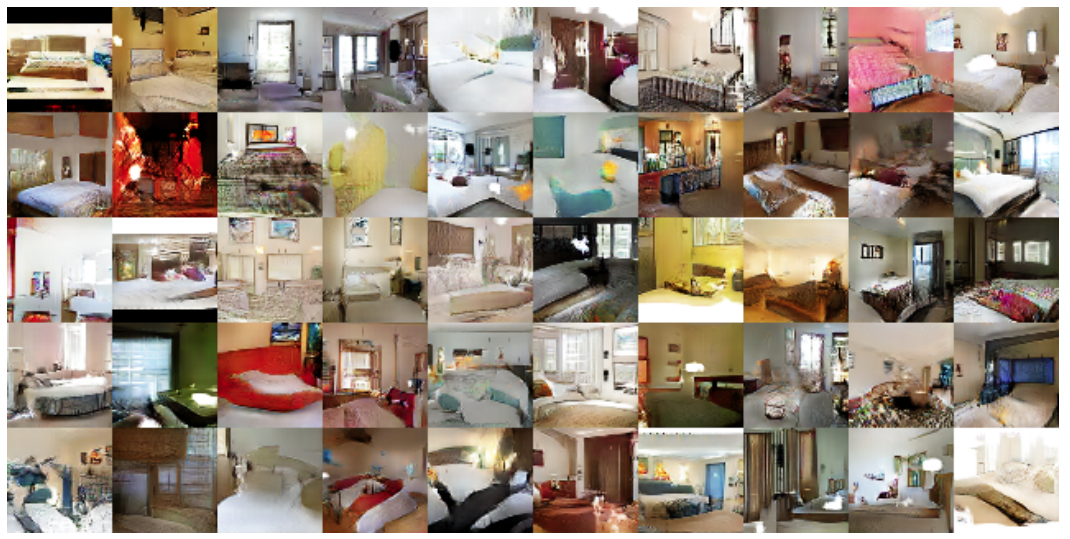
\includegraphics[width = 9in]{../images/GANDCa}}

\slidetwo{Unsupervised Representation Learning ... (DC GANS)}
{Radford et al., Nov. 2015}

\centerline{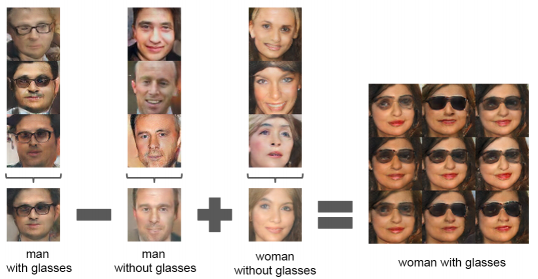
\includegraphics[width = 9in]{../images/ImageFeatures}}

\slide{Interpolated Faces}

[Ayan Chakrabarti, January 2017]

\centerline{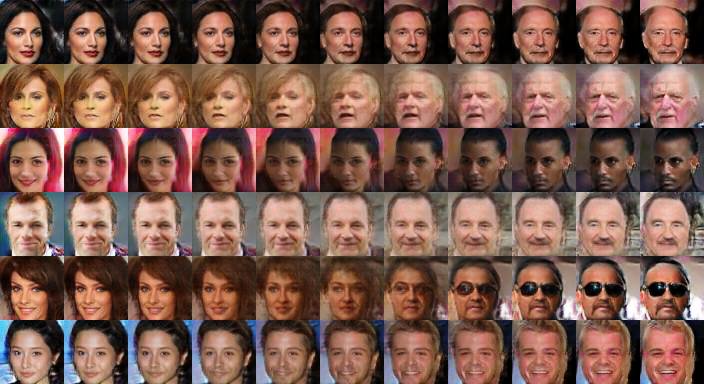
\includegraphics[height = 4.5in]{../images/interp}}

\slidetwo{Progressive Growing of GANs}{Karras et al., Oct. 2017}
\centerline{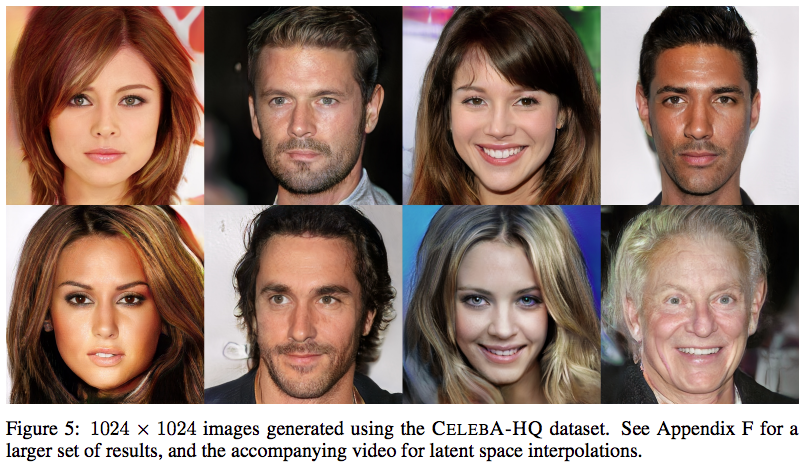
\includegraphics[height = 4.5in]{../images/GANproga}}

\slidetwo{Progressive Growing of GANs}{Karras et al., Oct. 2017}
\centerline{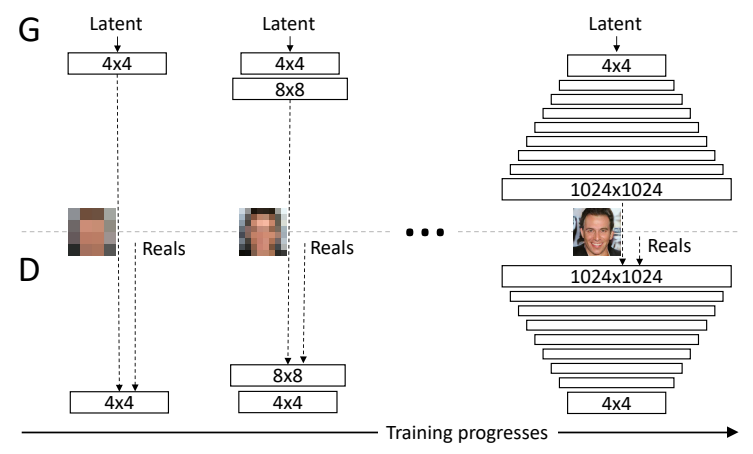
\includegraphics[height = 4.5in]{../images/GANprogb}}

\slidetwo{Progressive Growing of GANs}{Karras et al., Oct. 2017}
\centerline{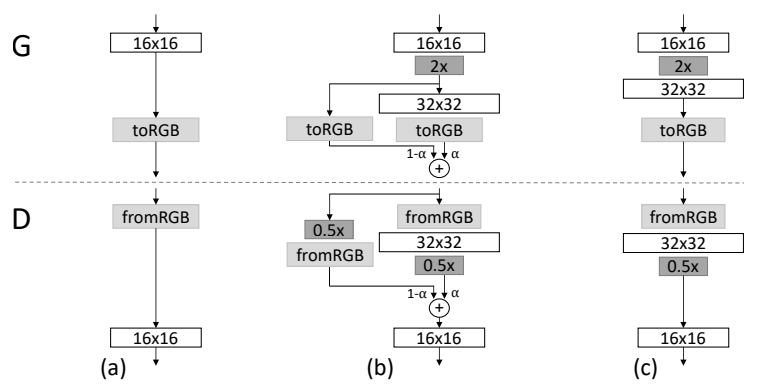
\includegraphics[height = 4.5in]{../images/GANprogc}}

\slide{Weakly Conditional GANs}

All unconditional distribution modeling methods apply to conditional distribution modeling.

$${\color{red} \Phi^* = \argmin_\Phi \; \max_\Psi \;\expectsub{i,x,y \sim (\popd\; \uplus \;\pop(x)p_\Phi(y|x))}
  {\ln P_\Psi(i|x,y)}}$$

By ``weakly conditional'' we mean that $x$ is discrete and carries little information ($H(x)$ is small).

\vfill
For example $x$ might be the class label associated with an image.


\slide{Early Unconditional GANs on ImageNet}

\centerline{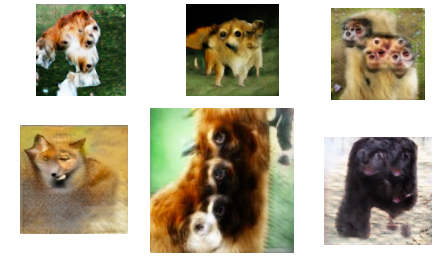
\includegraphics[height = 4.5in]{../images/BadGAN}}


\slidetwo{Large Scale GAN Training}{Brock et al., Sept. 2018}
\centerline{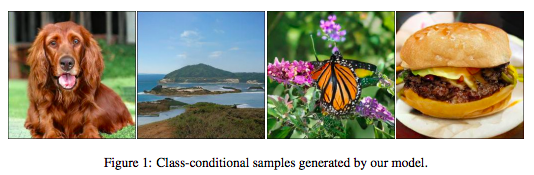
\includegraphics[width = 9in]{../images/GANclass}}

\vfill
This is a class-conditional GAN --- it is conditioned on the imagenet class label.

\vfill
This generates 512 X 512 images without using progressive training.
\slide{Issues}

\centerline{Mode Collapse}

\vfill
\centerline{Unstable Training}

\vfill
\centerline{Measuring Perfomance}

\ignore{

\slidetwo{Converting to Cross Entropy}{Goodfellow, 2014}

In Goodfellow's original paper he expressed a preference for cross entropy loss (the fundamental equation) over Jensen-Shannon loss.

$${\color{red} \Phi^* = \argmin_\Phi\;\mathrm{JSD}(\pop,P_\Phi)}$$

\centerline{vs.}
\vspace{-2ex}
$${\color{red} \Phi^* = \argmin_\Phi\;H(\pop,P_\Phi)}$$

{\color{red}
$$\begin{array}{lrcl}
\mathrm{GAN:} & \Phi^* & = & \argmin_\Phi\;\mathrm{JSD}(P_\Phi,\pop) \\
\\
\mathrm{GAN':} & \Phi^* & = & \argmin_\Phi H(\pop, P_\Phi) \\
\\
\mathrm{contrastiveGAN:} & \Phi^* & = & \argmin_\Phi KL(P_\Phi,\pop)
\end{array}$$
}

\vfill
He presented a modification to the GAN adversarial objective that yields cross-entropy loss rather than Jensen-Shanon loss.

\slidetwo{Converting to Cross Entropy}{Goodfellow, 2014}

{\color{red} $$\Psi^*(\Phi) = \argmin_\Psi \;\expectsub{(i,y) \sim (\mathrm{Pop}\; \uplus \;P_\Phi)}{- \ln P_\Psi(i|y)}$$}

\vfill
$$\mbox{Assume:}\;\;\; P_{\Psi^*}(1|y) = \frac{\mathrm{Pop}(y)}{\mathrm{Pop}(y) + P_\Phi(y)}$$

\vfill
\begin{eqnarray*}
  \mbox{Define:}\;\;\; {\color{red} f_{\Psi^*}(y)} & \doteq & \frac{P_{\Psi^*}(1|y)}{P_{\Psi^*}(-1|y)} \\
\\
& = & {\color{red} \frac{\mathrm{Pop}(y)}{P_\Phi(y)}}
\end{eqnarray*}

\slide{Converting to Cross Entropy}

{\huge
\begin{eqnarray*}
 {\color{red} \Phi^*}& = & {\color{red} \argmax_\Phi\;E_{y \sim \pop} \;f_{\Psi^*}(y)} \\
 \\
 {\color{red} \nabla_\Phi \; E_{y \sim P_\Phi}\;  f_{\Psi^*}(y)}  & = & \nabla _\Phi \sum_y\; P_\Phi(y) f_{\Psi^*}(y) \\
  \\
  & = & \sum_y \; P_\Phi(y) f_{\Psi^*}(y) \nabla_\Phi \ln P_\Phi(y) \\
  \\
  & = & \sum_y \;\mathrm{Pop}(y) \nabla_\Phi \ln P_\Phi(y) \\
  \\
  & = & E_{y \sim \mathrm{Pop}} \; \nabla_\Phi \ln P_\Phi(y) \\
  \\
  & = & {\color{red} \nabla_\Phi \; E_{y \sim \mathrm{Pop}} \;\ln P_\Phi(y)}
\end{eqnarray*}
}
}


\slide{Mode Collapse a.k.a Mode Dropping}

The generator distribution drops portions of the population.

\centerline{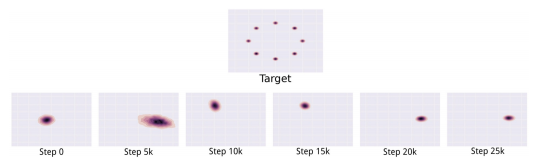
\includegraphics[width=9in]{../images/Unstable1}}

\slide{Unstable Training}

Joint SGD is not the same as nested max-min.

\vfill
Consider
$${\color{red} \max_x \; \min_y\; xy}$$

\vfill
A Nash equilibrium is $x= y = 0$.

\vfill
Simultaneous gradient flow yields

{\color{red} $$\frac{dx}{dt}  =  y \;\;\;\;\;\;\frac{dy}{dt} = -x$$}

\vfill
This goes in a circle.

\slide{Unstable Training}

The generator distribution drifts as the discriminator follows.

\centerline{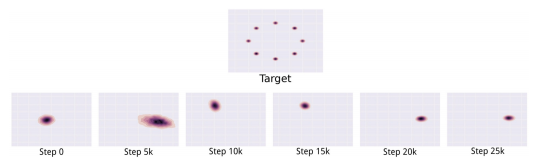
\includegraphics[width=9in]{../images/Unstable1}}

\slidetwo{Pros and Cons of GAN Evaluation Measures}{Borji, Oct 2018}

We would like a rate-distortion metric on distribution models.

\vfill
This has not yet been achieved for GANs.

\vfill
Evaluation of GANs always involves, at least in part, subjective judgments of naturalness.

\vfill
Sometimes automated metrics are also used.

\vfill
The above paper discusses various proposed automated metrics of GAN performance.  Current automated metrics are questionable.

\slide{}

\centerline{\bf Adversarial Discrimination as an Additional Loss}

\vfill
\vfill

\slide{Adversarial Discrimination as an Additional Loss}

$${\color{red} \Phi^* = \argmin_\Phi\;E_{(x,y) \sim \popd}\;\; ||y - \hat{y}(x)||^2\; +\; \lambda\; {\cal L}_{\mathrm{Discr}}(y,\hat{y}(x),x)}$$

\vfill
$${\cal L}_{\mathrm{Discr}}(y,\hat{y},x) = \max_\Psi \;E_{i,y' \sim \{y\}\uplus \{\hat{y}\}}\; \ln P_\Psi(i|y',x)$$

\slidetwo{Image-to-Image Translation (Pix2Pix)}
{Isola et al., Nov. 2016}

We assume a corpus of ``image translation pairs'' such as images paired with semantic segmentations.

\centerline{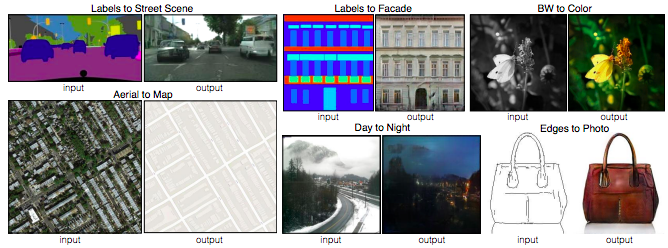
\includegraphics[width = 8.0in]{../images/cGAN0}}

\slide{Discrimination as an Additional Loss}

{\huge
$$\begin{array}{lrcl}
\mathrm{L1:} & \Phi^* & = & \argmin_\Phi\;E_{(x,y) \sim \popd}\;\; ||y - \hat{y}(x)||_1 \\
\\
\\
\mathrm{cGAN:} & \Phi^* & = & \argmin_\Phi\;E_{(x,y) \sim \popd}\;\; {\cal L}_{\mathrm{Discr}}(y,\hat{y}(x),x) \\
\\
\\
\mathrm{L1 + cGAN:} & \Phi^* & = & \argmin_\Phi\;E_{(x,y) \sim \popd}\;\; ||y - \hat{y}(x)||_1\; +\; \lambda\; {\cal L}_{\mathrm{Discr}}(y,\hat{y}(x),x)
\end{array}$$
}


$${\cal L}_{\mathrm{Discr}}(y,\hat{y},x) = \max_\Psi \;E_{i,y' \sim \{y\}\uplus \{\hat{y}\}}\; \ln P_\Psi(i|y',x)$$
\slidetwo{Image-to-Image Translation (Pix2Pix)}
{Isola et al., Nov. 2016}

\centerline{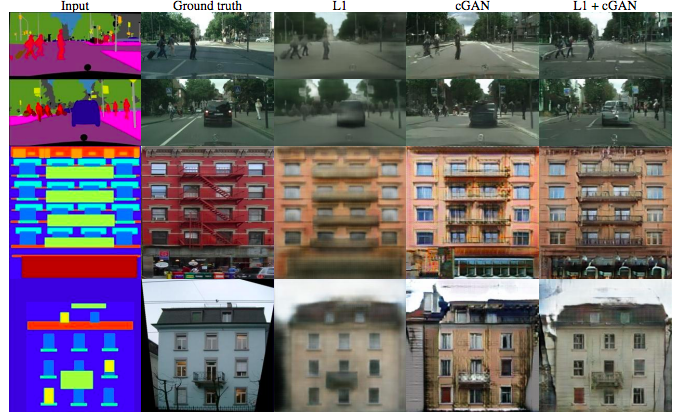
\includegraphics[height = 4.5in]{../images/cGAN1}}

\slide{Arial Photo to Map and Back}

\centerline{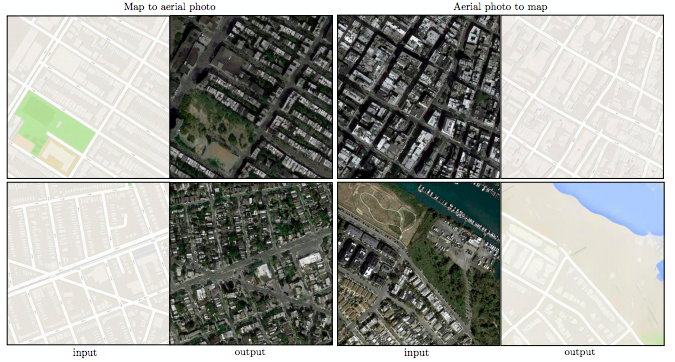
\includegraphics[width = 8.0in]{../images/cGAN2}}

\slide{Semantic Segmentation}

\centerline{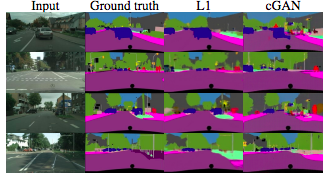
\includegraphics[width = 8.0in]{../images/cGAN4}}

\ignore{
\slidetwo{Unpaired Image-to-Image Translation (Cycle GANs)}{Zhu et al., March 2017}

We have two corpora of images, say images of zebras and unrelated images of horses, or photographs and unrelated paintings by Monet.

\vfill
We want to construct translations between the two classes.

\centerline{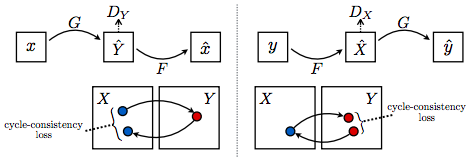
\includegraphics[width = 8.0in]{../images/Cycle2}}

\slide{Cycle Gans}

\centerline{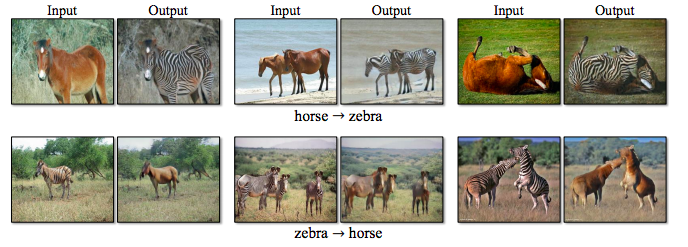
\includegraphics[width = 11.0in]{../images/Cycle3}}

\slide{Cycle Gans}

\centerline{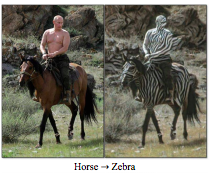
\includegraphics[width = 6.0in]{../images/Cycle4}}

\slidetwo{Unsupervised Machine Translation (UMT)}
         {Lample et al, Oct. 2017, also Artetxe et al., Oct. 2017}

\centerline{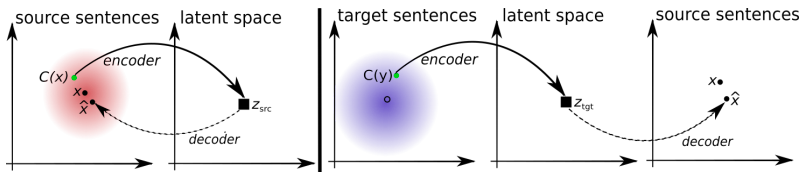
\includegraphics[width = 10.0in]{../images/Cycle5}}
}

\slidetwo{Feature Alignment by Discrimination}{Text to Speech (Saito et al. Sept. 2017)}

\centerline{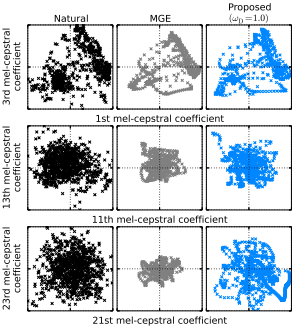
\includegraphics[width = 2.0in]{../images/Txt2spchGAN}}

\vfill
Minimum Generation Error (MGE) uses {\color{red} perceptual distortion} ---
a distance between the feature vector of the generated sound wave and the
feature vector of the original.

\vfill
{\color{red}Perceptual Naturalness} can be enforced by a feature discrimination loss.

\slidetwo{Adversarial Discriminative Domain Adaptation}{Tzeng et al. Feb. 2017}

\centerline{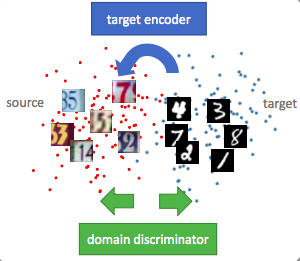
\includegraphics[width = 4.0in]{../images/AdvDomainAdapt}}

A feature discrimination loss can be used to align source and target features.

\slide{Comments}

\vfill
I predict that in a few years adversarial discrimination will be limited to enforcing perceptual naturalness in the generation of sounds and images.

\vfill
Cooperative discrimination seems more useful for predictive tasks.  Cooperative discrimination has been effective in pretraining.
We consider pretraining in the next lecture.
\slide{END}

}
\end{document}
